\begin{figure}[ht!]
  \centering
  \begin{subfigure}[t]{0.4\textwidth}
    \centering
    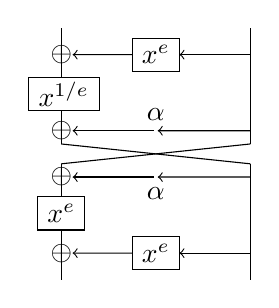
\begin{tikzpicture}[xscale=0.6, yscale=0.42]
      % TOP PART
      % -- cube
      \draw (-0.5, +2.5) rectangle node[pos=0.5]{$x^e$} (+0.5, +3.5);
      % -- cube inverse
      \draw (-1.2, +1.3) rectangle node[pos=0.5]{$x^{1/e}$} (-2.7, +2.3);
      % -- alpha multiplication
      \draw (+0.0, +0.7) node[inner sep=0](mult0){$\fmult$} ;
      \draw (+0.0, +1.2) node[inner sep=0]{$\alpha$} ;
      % -- XORs
      \draw (-2.0, +3.0) node[inner sep=0](xor0){$\oplus$} ;
      \draw (-2.0, +0.7) node[inner sep=0](xor1){$\oplus$} ;
      % -- wires
      \draw (+2.0, +3.8) -- (+2.0, +0.3);
      \draw (-2.0, +3.8) -- (-2.0, +2.3);
      \draw[->] (+2.0, +3.0) -- (+0.5, +3.0);
      \draw[->] (-0.5, +3.0) -- (xor0);
      \draw[->] (+2.0, +0.7) -- (mult0);
      \draw[->] (mult0) -- (xor1);
      \draw (-2.0, +1.3) -- (-2.0, +0.3);
      % MIDDLE WIRING
      \draw (+2.0, +0.3) -- (-2.0, -0.3);
      \draw (-2.0, +0.3) -- (+2.0, -0.3);
      % BOTTOM PART
      % -- cube (xored)
      \draw (-0.5, -2.5) rectangle node[pos=0.5]{$x^e$} (+0.5, -3.5);
      % -- cube
      \draw (-1.5, -1.3) rectangle node[pos=0.5]{$x^{e}$} (-2.5, -2.3);
      % -- alpha multiplication
      \draw (+0.0, -0.7) node[inner sep=0](mult1){$\fmult$} ;
      \draw (+0.0, -1.2) node[inner sep=0]{$\alpha$} ;
      % -- XORs
      \draw (-2.0, -3.0) node[inner sep=0](xor2){$\oplus$} ;
      \draw (-2.0, -0.7) node[inner sep=0](xor3){$\oplus$} ;
      % -- wires
      \draw (+2.0, -3.8) -- (+2.0, -0.3);
      \draw (-2.0, -3.8) -- (-2.0, -2.3);
      \draw[->] (+2.0, -3.0) -- (+0.5, -3.0);
      \draw[->] (-0.5, -3.0) -- (xor2);
      \draw[->] (+2.0, -0.7) -- (mult1);
      \draw[->] (mult1) -- (xor3);
      \draw (-2.0, -1.3) -- (-2.0, -0.3);
    \end{tikzpicture}  
    \FigDef{open-butterfly}{Open (bijective) butterfly $\openB{e}{\alpha}$.}
  \end{subfigure}
  \hspace{0.2cm}
  \begin{subfigure}[t]{0.55\textwidth}
    \centering
    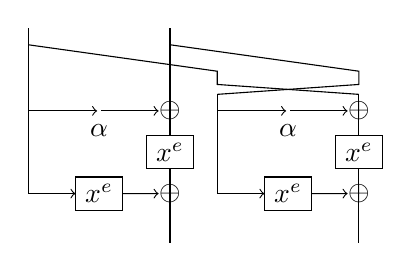
\begin{tikzpicture}[xscale=0.6, yscale=0.42]
      % LEFT PART
      % -- alpha multiplication
      \draw (-2.5, +0.0) node[inner sep=0](mult_l){$\fmult$} ;
      \draw (-2.5, -0.6) node[inner sep=0]{$\alpha$} ;
      \draw (-1.0, +0.0) node[inner sep=0](xor_ml){$\oplus$} ;
      % -- cube
      \draw (-1.5, -1.75) rectangle node[pos=0.5]{$x^e$} (-0.5, -0.75);
      % -- cube (xored)
      \draw (-3.0, -3.0) rectangle node[pos=0.5]{$x^e$} (-2.0, -2.0);
      \draw (-1.0, -2.5) node[inner sep=0](xor_cl){$\oplus$} ;
      % -- wiring
      \draw (-4.0, +0.5) -- (-4.0, -2.5);
      \draw (-1.0, +0.5) -- (-1.0, -0.75);
      \draw (-1.0, -1.75) -- (-1.0, -3.0);
      \draw[->] (-4.0, +0.0) -- (mult_l);
      \draw[->] (mult_l) -- (xor_ml);
      \draw[->] (-4.0, -2.5) -- (-3.0, -2.5);
      \draw[->] (-2.0, -2.5) -- (xor_cl);
      % RIGHT PART
      % -- alpha multiplication
      \draw (+1.5, +0.0) node[inner sep=0](mult_l){$\fmult$} ;
      \draw (+1.5, -0.6) node[inner sep=0]{$\alpha$} ;
      \draw (+3.0, +0.0) node[inner sep=0](xor_ml){$\oplus$} ;
      % -- cube
      \draw (+2.5, -1.75) rectangle node[pos=0.5]{$x^e$} (+3.5, -0.75);
      % -- cube (xored)
      \draw (+1.0, -3.0) rectangle node[pos=0.5]{$x^e$} (+2.0, -2.0);
      \draw (+3.0, -2.5) node[inner sep=0](xor_cl){$\oplus$} ;
      % -- wiring
      \draw (+0.0, +0.5) -- (+0.0, -2.5);
      \draw (+3.0, +0.5) -- (+3.0, -0.75);
      \draw (+3.0, -1.75) -- (+3.0, -3.0);
      \draw[->] (+0.0, +0.0) -- (mult_l);
      \draw[->] (mult_l) -- (xor_ml);
      \draw[->] (+0.0, -2.5) -- (+1.0, -2.5);
      \draw[->] (+2.0, -2.5) -- (xor_cl);
      % WIRING
      \draw (-4.0, +2.5) -- (-4.0, +0.5);
      \draw (-1.0, +2.5) -- (-1.0, +0.5);
      \draw (-4.0, +2.0) -- (+0.0, +1.2) -- (+0.0, +0.8) -- (+3.0, +0.5);
      \draw (-1.0, +2.0) -- (+3.0, +1.2) -- (+3.0, +0.8) -- (+0.0, +0.5);
      \draw (-1.0, -3.0) -- (-1.0, -4.0);
      \draw (+3.0, -3.0) -- (+3.0, -4.0);
    \end{tikzpicture}  
    \FigDef{closed-butterfly}{Closed (non-bijective) butterfly $\closedB{e}{\alpha}$.}
  \end{subfigure}
  \FigDef{butterflies}{The two kinds of butterfly structure.}
\end{figure}

